\begin{figure}[ht]
\centering
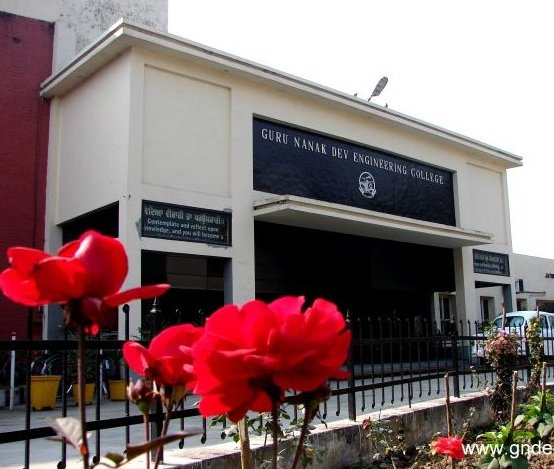
\includegraphics[scale=0.5]{input/images/gndec.jpg}
\caption{Guru Nanak Dev Engineering College}
\end{figure}
\hspace{-1.7em} I had my Six Month Industrial Training at TCC-Testing And Consultancy Cell under the guidance of Dr. H.S.Rai Dean TCC, GNDEC Ludhiana. Guru Nanak Dev Engineering College was established by the Nankana
Sahib Education Trust Ludhiana. The Nankana Sahib Education Trust i.e NSET
was founded in memory of the most sacred temple of Sri Nankana Sahib, birth place
of Sri Guru Nanak Dev Ji. With the mission of Removal of Economic Backwardness
through Technology Shiromani Gurudwara Parbandhak Committee i.e SGPC started a
Poly technical was started in 1953 and Guru Nanak Dev Engineering College was established in 1956.\\


The main goal of this institute is:
\begin{itemize}
\item To build and promote teams of experts in the upcoming specialisations.
\item To promote quality research and undertake research projects keeping in view their
relevance to needs and requirements of technology in local industry.
\item To achieve total financial independence.
\item To start online transfer of knowledge in appropriate technology by means of establishing multipurpose resource centres.
\end{itemize}
\section{Testing and Consutancy Cell}

Testing and Consultancy Cell was established in the year 1979 with a basic aim to produce
quality service for technical problems at reasonable and affordable rates as a service to society
in general and Engineering fraternity in particular.\\

Consultancy Services are being rendered by various Departments of the College to the
industry, Sate Government Departments and Entrepreneurs and are extended in the form of
expert advice in design, testing of materials \& equipment, technical surveys, technical audit,
calibration of instruments, preparation of technical feasibility reports etc.
This consultancy cell of the college has given a new dimension to the development
programmers of the College. Consultancy projects of over Rs. one crore are completed by the
Consultancy cell during financial year 2009-10. \\

Ours is a pioneer institute providing Consultancy Services in the States of Punjab, Haryana,
Himachal, J\&K and Rajasthan. Various Major Clients of the Consultancy Cell are as under:\\
\begin{itemize}
\item Northern Railway, Govt. of India
\item Indian Oil Corporation Ltd.
\item Larson \& Turbo.
\item Multi National Companies like AFCON \& PAULINGS.
\item Punjab Water Supply \& Sewage Board
\end{itemize}

